\begin{recipe}{蝴蝶海参}

\ingredients

\ingredient{刺参(张片好的参均可)}{二两五}
\ingredient{冬笋}{一两}
\ingredient{干豆粉}{二钱}
\ingredient{鲤鱼(做糁)}{八两}
\ingredient{鸡蛋清}{二个}
\ingredient{特级清汤}{一斤半}
\ingredient{胡椒}{二分}
\ingredient{火腿}{一钱}
\ingredient{黑芝麻}{数十粒}
\ingredient{肥膘猪肉}{一两五}
\ingredient{盐}{八分}

\preparation

\step 刺参先用开水泡发,洗净内外粗渣杂质,入炒锅内加清水以微火煨𤆵(约二十分
钟);捞起用刀片成二分厚的薄片,再切成一寸二分宽、一寸长,共二十四片,然后用刀
尖雕成蝴蝶形。(如图\,\ref{用海参雕成的蝴蝶形}\,)

\begin{wrapfigure}[7]{l}{9em}%
\centering%
\vspace{-.6875\baselineskip}%

\includegraphics[scale=1]{illustration-008.pdf}%
\vspace{-.1875\baselineskip}%
\caption{用海参雕成的蝴蝶形}%
\label{用海参雕成的蝴蝶形}%
\end{wrapfigure}

\step 鲤鱼去鱗、去头尾和刺,取净肉剁为细茸;猪肥膘肉洗净,剁为细茸;加蛋清一个
半,胡椒、盐共入碗中,加清水少许搅为“鱼糁”;蛋清半个加豆粉搅匀成蛋清豆粉。

\step 蝴蝶海参片投入三级清汤中,加盐煮约十分钟,而后使之入味,捞出铺于盘上以净
布揩干,逐片把白色一面用蛋清豆粉抹匀,再用刀尖沾碗内的鱼糁放在蝴蝶片的中央,成
为蝴蝶的腹部(如图\,\ref{中央涂上鱼糁为蝴蝶腹部}\,);每片用糁长一寸、宽三分、
厚四分,形如橄榄,随后用手沾清水涂抹光滑。

\step 冬笋去壳,切成六分长的细丝四十八根,其余均切为三分长的短丝;火腿切成三分
长的细丝;用手把火腿丝和笋丝相间地横镶于腹部上面,另外,以两根笋丝镶于每个蝴蝶
头部左右为触须,用细竹签前端沾水,蘸黑芝麻插入须侧左右各一粒为蝴蝶眼(如
图\,\ref{蝴蝶海参}\,)。

\begin{figure}[h]
\vspace{-.25\baselineskip}%
\parbox{14.75em}{%
        \vspace{-.1875\baselineskip}%
        \hspace{2em}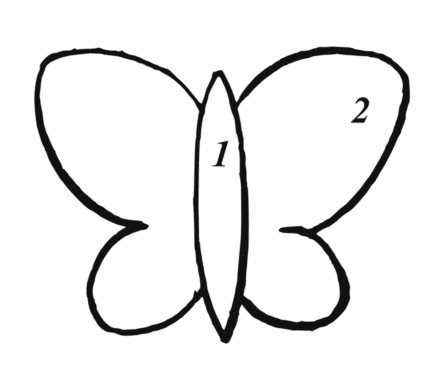
\includegraphics[scale=1]{illustration-009.pdf}%
        \vspace{-.4375\baselineskip}%
        \caption{中央涂上鱼糁为蝴蝶腹部}
		\label{中央涂上鱼糁为蝴蝶腹部}
        \begingroup%
        \small%
        \noindent%
        \null\hspace{4em}1. 鱼糁;2. 海参片
        \endgroup%
}%
\begin{minipage}{10.75em}
        
\includegraphics[scale=1]{illustration-010.pdf}%
        \caption{蝴蝶海参}
        \label{蝴蝶海参}
        \begingroup%
        \small%
        \noindent%
        \null\hspace{1.5em}1. 火腿丝;2. 冬笋丝;\\
        \null\hspace{1.5em}3. 黑芝麻;4. 海参片
        \endgroup%
\end{minipage}
\vspace{-.25\baselineskip}%
\end{figure}%
\vbadness=10000%

\step 作好的蝴蝶形海参摆于盘中,入笼蒸三分钟,定形时取出放汤碗内,碗内加特级清
汤、胡椒、盐即成,“蝴蝶”由于糁的关系,每个均浮于汤面。

\features

此菜系汤菜,汤鲜美可口,蝴蝶形状美观。

\end{recipe}

% vim: filetype=tex noautoindent nojoinspaces
% vim: fileencoding=utf-8 formatoptions+=m
% vim: textwidth=78 tabstop=4 shiftwidth=4 softtabstop=4
